\newchapter{phaseMons}{Phase Monitor Performance}

This is the introductory text.

Mon1 = first mon in CT
Mon2 = second mon in CT
Mon3 = mon in TBL

Mon1/Mon2 = upstream phase
Mon3 = downstream phase

\newsection{monElectronics}{Phase Monitor Electronics}

Hybrid - remove dipole (position dependent) mode. 19dB below monopole mode for 1mm offset (11\% amplitude). 1mm beam offset = 2.8 degrees phase offset. 180 degree hybrids to remove. Additional 20 dB attenuation in dipole mode.

Bunch length sensitivity: more sensitive to variation in bunch length for longer variations. 5mm bunch length - 50\% amplitude output compared to 0mm. With 1mm bunches 16\% variation in bunch length needed to cause 1\% change in output voltage.

LO should have 5fs stability? What is the source of the LO?

Mixer output
\begin{align}
RF(t) &= A_{RF}(t)\cos[\omega_{RF} t + \phi(t)] \\
LO(t) &= A_{LO}\cos[\omega_{LO} t]
\end{align}
mixer multiplies
\begin{align}
\mathrm{Mixer}(t) &= RF(t) \times LO(t) \\
\mathrm{Mixer}(t) &= A_{RF}(t)A_{LO}\cos[\omega_{RF} t + \phi(t)]\cos[\omega_{LO} t]
\end{align}
trig identities
\begin{equation}
\mathrm{Mixer}(t) = \frac{A_{RF}(t)A_{LO}}{2}\left\lbrace\cos[(\omega_{LO} + \omega_{RF})t + \phi(t)] + \cos[(\omega_{LO} - \omega_{RF})t + \phi(t)]\right\rbrace
\end{equation}
filter high frequency
\begin{equation}
\mathrm{Mixer}(t) = \frac{A_{RF}(t)A_{LO}}{2}\cos[(\omega_{LO} - \omega_{RF})t + \phi(t)]
\label{e:mixOutAnyFreq} 
\end{equation}
LO frequency and RF frequency are the same
\begin{equation}
\mathrm{Mixer}(t) = \frac{A_{RF}(t)A_{LO}}{2}\cos[\phi(t)]
\label{e:mixOutSameFreq} 
\end{equation}
Diode used to measure \(A_{RF}\)
\begin{equation}
\mathrm{Diode}(t) = bA_{RF}(t)^2
\end{equation}
The phase can be reconstructed by
\begin{align}
&\frac{\mathrm{Mixer}(t)}{\sqrt{\mathrm{Diode}(t)}} = A\cos[\phi(t)] \\
&\phi(t) = \arccos\left[\frac{\mathrm{Mixer(t)}}{A\sqrt{\mathrm{Diode(t)}}}\right]
\label{e:phaseRecIdeal} 
\end{align}

Beam/monitor frequency is 11.994 GHz.

Performance limited by:
Device non-linearity -- normally better for lower input power
Signal to noise -- better for high power
Therefore, split signal to 8 mixers -- low input power to each one -- to reduce effect of non-linearities. Then sum up results of each mixer to improve signal to noise.

Monitor -> attenuator? -> Hybrid sum -> attenuator? -> attenuator in gallery -> mixer RF input
LO -> phase shifter -> multiplier -> amplifier -> mixer LO input
Mixer output -> attenuator -> amplifier -> SiS OR -> attenuator->FONT
Diode output -> SiS/FONT

Latest power measurements:
Mon1 24.6 dBm
Mon2 26.8 dBm
Mon3 24.5 dBm
LO1 22.6 dBm
LO2 23.6 dBm
LO3 25.5 dBm

\newsection{monSigResponse}{Signal Response Measurements}

Measurements have been taken using a 12~GHz signal generator to determine the performance of the three sets of phase monitor electronics independently from the phase monitors themselves. In particular, these tests were focused on identifying the saturation and cross-talk characteristics of the output mixer and diode signals.

\subsection{Experimental Setup}
\label{ss:sigGenSetup}

The only change to the setup shown in Figure~[REF] made for these tests is that the beam induced signal from the phase monitors usually connected to the RF port of the mixers is replaced by the output from a 12~GHz signal generator. To be able to reach the same input power levels as the beam signals the signal generator output is amplified using a [TODO:amplifierInfo]. This allows the input power to the mixers to be varied in a wide range between 0 and 33dBm, or between 0.2 and 12.6~V. The precise power sent to the mixer is verified between each measurement using a power meter. 

The diode outputs were amplified during these tests (using the same amplifier introduced in Section~\ref{ss:sisNoise}) by a factor 10 in voltage to reduce digitiser noise in the measurement. The non-amplified peak diode output is therefore 170~mV, rather than the 1.7~V seen in the plots in this section. The \(\pm500\)~mV mixer outputs have not been amplified.

There are some differences between the properties of the generated signal and the beam signal that would be used in normal operation. Firstly, unlike the pulsed beam signal the used generated signal is continuous. It has been verified that the response of the mixers is equivalent for both the continuous and pulsed signals, at least in terms of output power and saturation levels [REF]. The cross-talk properties are difficult to characterise with beam based measurements alone.

Secondly, the phase of the generated signal does not vary with time, compared to the beam signal which has a large \(\sim40^\circ\) phase sag along the pulse and much larger phase jitter. If the signal generator was used at the same frequency as the beam and LO signals, 11.994~GHz, the mixer output would therefore be constant as it depends only on the static phase as per Equation~\ref{e:mixOutSameFreq}. Instead, a generated signal with a slightly lower frequency of 11.991~GHz has been used. From Equation~\ref{e:mixOutAnyFreq} it can be seeen that in this case the mixer output voltage is sinusoidal, with a frequency equal to the frequency difference between the LO and RF inputs -- or \(11.994-11.991\)~GHz = 3~MHz with the setup used here. This has the benefit of being able to see the response of the electronics to all input phases in one measurement, rather than having to take multiple measurements varying the LO phase shifter between each one.

\subsection{Results}
\label{ss:sigGenResults}

Figures~\ref{f:sigGenAllMix1}--\ref{f:sigGenAllDio3} show the mixer and diode outputs for all three sets of electronics at each of the input power levels sent from the signal generator.

\begin{figure}
  \centering
  \includegraphics[width=0.9\textwidth]{Figures/phaseMons/Mixer1_AllPowerLevels}
  \caption{Response of Mixer 1 to signal generator input.}
  \label{f:sigGenAllMix1}
  \includegraphics[width=0.9\textwidth]{Figures/phaseMons/Diode1_AllPowerLevels}
  \caption{Response of Diode 1 to signal generator input.}
  \label{f:sigGenAllDio1}
\end{figure}

\begin{figure}
  \centering
  \includegraphics[width=0.9\textwidth]{Figures/phaseMons/Mixer2_AllPowerLevels}
  \caption{Response of Mixer 2 to signal generator input.}
  \label{f:sigGenAllMix2}
  \includegraphics[width=0.9\textwidth]{Figures/phaseMons/Diode2_AllPowerLevels}
  \caption{Response of Diode 2 to signal generator input.}
  \label{f:sigGenAllDio2}
\end{figure}

\begin{figure}
  \centering
  \includegraphics[width=0.9\textwidth]{Figures/phaseMons/Mixer3_AllPowerLevels}
  \caption{Response of Mixer 3 to signal generator input.}
  \label{f:sigGenAllMix3}
  \includegraphics[width=0.9\textwidth]{Figures/phaseMons/Diode3_AllPowerLevels}
  \caption{Response of Diode 3 to signal generator input.}
  \label{f:sigGenAllDio3}
\end{figure}

fits of mixer response

\subsection{Linearity and Saturation}
\label{ss:monSaturation}

\begin{figure}
  \centering
  \includegraphics[width=0.9\textwidth]{Figures/phaseMons/MixerVsVolts}
  \caption{Mixer output voltage vs. input voltage.}
  \label{f:MixerVsVolts}
\end{figure}

\begin{figure}
  \centering
  \includegraphics[width=0.9\textwidth]{Figures/phaseMons/LinFitMixerVsVolts}
  \caption{Linear fit to mixer output voltage vs. input voltage.}
  \label{f:LinFitMixerVsVolts}
\end{figure}

\begin{figure}
  \centering
  \includegraphics[width=0.9\textwidth]{Figures/phaseMons/SqrtDiodeVsVolts}
  \caption{sqrt(Diode) vs. input voltage.}
  \label{f:SqrtDiodeVsVolts}
\end{figure}

\begin{figure}
  \centering
  \includegraphics[width=0.9\textwidth]{Figures/phaseMons/LinFitSqrtDiodeVsVolts}
  \caption{Fit to sqrt(Diode) vs. input voltage.}
  \label{f:LinFitSqrtDiodeVsVolts}
\end{figure}

\subsection{Cross-Talk}
\label{ss:crossTalk}

\begin{figure}
  \centering
  \includegraphics[width=0.9\textwidth]{Figures/phaseMons/RelativeMixerXTalkvsPower}
  \caption{Relative amplitude vs. input power of cross-talk on the mixer from the diode.}
  \label{f:RelativeMixerXTalkvsPower}
\end{figure}

\begin{figure}
  \centering
  \includegraphics[width=0.9\textwidth]{Figures/phaseMons/RelativeDiodeXTalkVsPower}
  \caption{Relative amplitude vs. input power of cross-talk on the diode from the mixer.}
  \label{f:RelativeDiodeXTalkVsPower}
\end{figure}

fits to diode cross-talk

\newsection{monCalibrations}{Calibrations}

\subsection{Procedure}
\label{ss:calProcedure}

\subsection{Single Sample Results}
\label{ss:calSingSamp}

\subsection{Multi-Sample Results}
\label{ss:calMultiSamp}

\newsection{digNoise}{Digitiser Noise}

\subsection{On FONT5 Board}
\label{ss:font5Noise}

\subsection{On SiS Digitiser}
\label{ss:sisNoise}

\newsection{shifters}{Phase Shifter Noise}

\subsection{Digital Phase Shifters}
\label{ss:digShiftNoise}

\begin{figure}
  \centering
  \includegraphics[width=0.9\textwidth]{Figures/phaseMons/PhMon_HistDig1}
  \caption{Dig shifter 1.}
  \label{f:PhMon_HistDig1}
\end{figure}

\begin{figure}
  \centering
  \includegraphics[width=0.9\textwidth]{Figures/phaseMons/PhMon_HistDig2}
  \caption{Dig shifter 2.}
  \label{f:PhMon_HistDig2}
\end{figure}

\begin{figure}
  \centering
  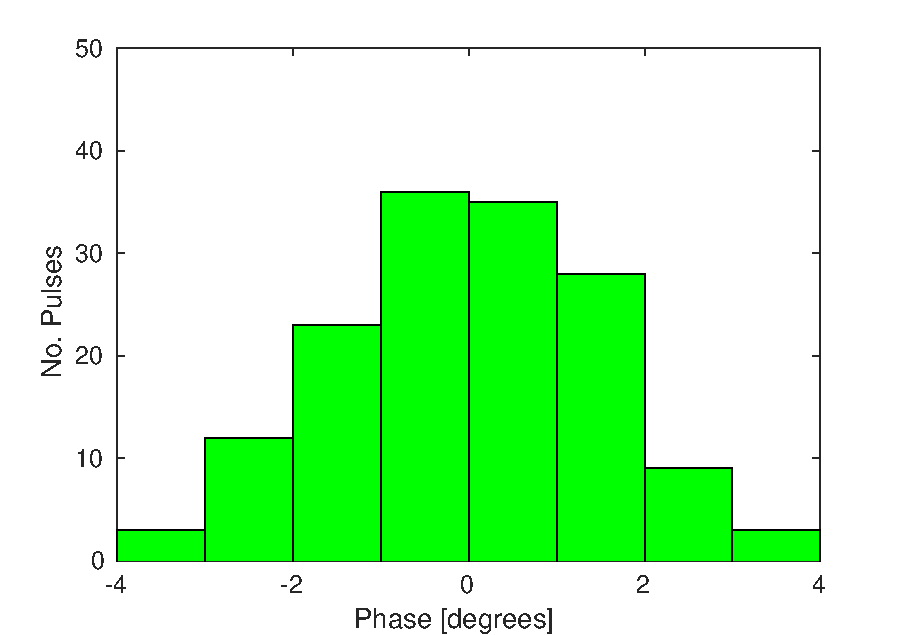
\includegraphics[width=0.9\textwidth]{Figures/phaseMons/PhMon_HistDig3}
  \caption{Dig shifter 3.}
  \label{f:PhMon_HistDig3}
\end{figure}

\subsection{Mechanical Phase Shifters}
\label{ss:mechShiftNoise}

\begin{figure}
  \centering
  \includegraphics[width=0.9\textwidth]{Figures/phaseMons/PhMon_HistMech}
  \caption{Mech shifter.}
  \label{f:PhMon_HistMech}
\end{figure}

\newsection{resolution}{Resolution}

Single sample.

(Multi-sample)

Sample averaging.

Impact for phase correlations.

vs. shifter setting

\begin{figure}
  \centering
  \includegraphics[width=0.9\textwidth]{Figures/phaseMons/PhMon_Resolution}
  \caption{Resolution.}
  \label{f:PhMon_Resolution}
\end{figure}

\newsection{monLinearity}{Linearity}

\newsection{monBandwidth}{Bandwidth}

\newsection{monPosition}{Dependence on Position}








